\documentclass[a4paper,12pt]{article}
\usepackage{amsmath,amssymb,amsfonts,amsthm}
\usepackage{tikz}
\usepackage [utf8x] {inputenc}
\usepackage [T2A] {fontenc} 
\usepackage[russian]{babel}
\usepackage{cmap} 

% Так ссылки в PDF будут активны
\usepackage[unicode]{hyperref}

% вы сможете вставлять картинки командой \includegraphics[width=0.7\textwidth]{ИМЯ ФАЙЛА}
% получается подключать, как минимум, файлы .pdf, .jpg, .png.
\usepackage{graphicx}
% Если вы хотите явно указать поля:
\usepackage[margin=1in]{geometry}
% Или если вы хотите задать поля менее явно (чем больше DIV, тем больше места под текст):
% \usepackage[DIV=10]{typearea}

\usepackage{fancyhdr}

\newcommand{\bbR}{\mathbb R}%теперь вместо длинной команды \mathbb R (множество вещественных чисел) можно писать короткую запись \bbR. Вместо \bbR вы можете вписать любую строчку букв, которая начинается с '\'.
\newcommand{\eps}{\varepsilon}
\newcommand{\bbN}{\mathbb N}
\newcommand{\dif}{\mathrm{d}}

\newtheorem{Def}{Определение}


\pagestyle{fancy}
\makeatletter % сделать "@" "буквой", а не "спецсимволом" - можно использовать "служебные" команды, содержащие @ в названии
\fancyhead[L]{\footnotesize Термодинамика и молекулярная физика}%Это будет написано вверху страницы слева
\fancyhead[R]{\footnotesize ФМХФ МФТИ}
\fancyfoot[L]{\footnotesize \@author}%имя автора будет написано внизу страницы слева
\fancyfoot[R]{\thepage}%номер страницы —- внизу справа
\fancyfoot[C]{}%по центру внизу страницы пусто

\renewcommand{\maketitle}{%
	\noindent{\bfseries\scshape\large\@title\ \mdseries\upshape}\par
	\noindent {\large\itshape\@author}
	\vskip 2ex}
\makeatother
\def\dd#1#2{\frac{\partial#1}{\partial#2}}


\title{1.3.3 \\ Определение вязкости воздуха по скорости течения через тонкие трубки} 
\author{Егор Берсенев} 
\date{22 марта 2016 г.}

\begin{document}
	\maketitle
	\section{Цель работы}
		\begin{enumerate}
			\item Экспериментально выявить участок сформированного течения.
			\item Определить режимы ламинарного и турбулентного течения.
			\item Определить число Рейнольдса.
		\end{enumerate}
	\section{Оборудование}
		Металлические трубки, укрепленные на горизонтальной подставке, газовый счетчик, микроманометр ММН, U-образная трубка, секундомер.
	\section{Теоретическая часть}
		Рассмотрим движение вязкой жидкости по трубке круглого сечения. При малых скоростях потока движение оказывается ламинарным, скорости частиц меняются по радиусу и направлены вдоль оси трубки. С увеличением скорости течение становится турбулентным, и слои перемешиваются. При турбулентном движении скорость в каждой точке быстро меняет величину и направление, сохраняется только средняя  величина скорости.
		
		Характер движения газа в трубке определяется числом Рейнольдса:
		\begin{equation}
			Re = \frac{vr\rho}{\eta},
		\end{equation}
		где $v$ --- скорость потока, $r$ --- радиус трубки, $\rho$ --- плотность движущейся среды, $\eta$ --- вязкость. В гладких трубах круглого сечения переход от ламинарного движения к турбулентному происходит примерно при $Re \sim 1000$.
		При ламинарном течении объем газа V, протекающий за время $t$ по трубе длины $l$, определяется формулой Пуазейля:
		\begin{equation}
			Q_V = \frac{\pi r^4}{8l\eta}\left(P_1-P_2\right)
		\end{equation}
		Отметим условия применимости формулы $(2)$. Необходимо чтобы с достаточным запасом выполнялось неравенство $Re < 1000$. Также необходимо, чтобы не менялся удельный объем газа. Для жидкости это выполняется всегда, а для газа только в том случае, если перепад давлений вдоль трубки мал по сравнению с самим давлением. В нашем случае давление газа равно атмосферному ($10^3$ см. вод. ст.), а перепад давлений составляет не более 10 см. вод. ст. Формула (2) выводится для участков трубы, на которых закон распределения скоростей не меняется вдоль потока. При втекании газа в трубку из большого резервуара скорости слоев в начале постоянны по всему сечению, но по мере продвижения по трубке картина распределения скоростей меняется и устанавливается Пуазейлевский профиль скоростей. Этот профиль устанавливается на некотором расстоянии $a$ от входа в трубку, которое зависит от радиуса трубки $r$ и числа Рейнольдса по формуле
		\begin{equation}
			a \sim 0.2r\cdot Re
		\end{equation}
		Градиент давления на участке формирования потока оказывается большим, чем на участке с установившимся ламинарным течением, что позволяетразделить эти участки экспериментально. Формула (3) дает возможность оценить  длину участка формирования.
	\section{Устройство установки}
		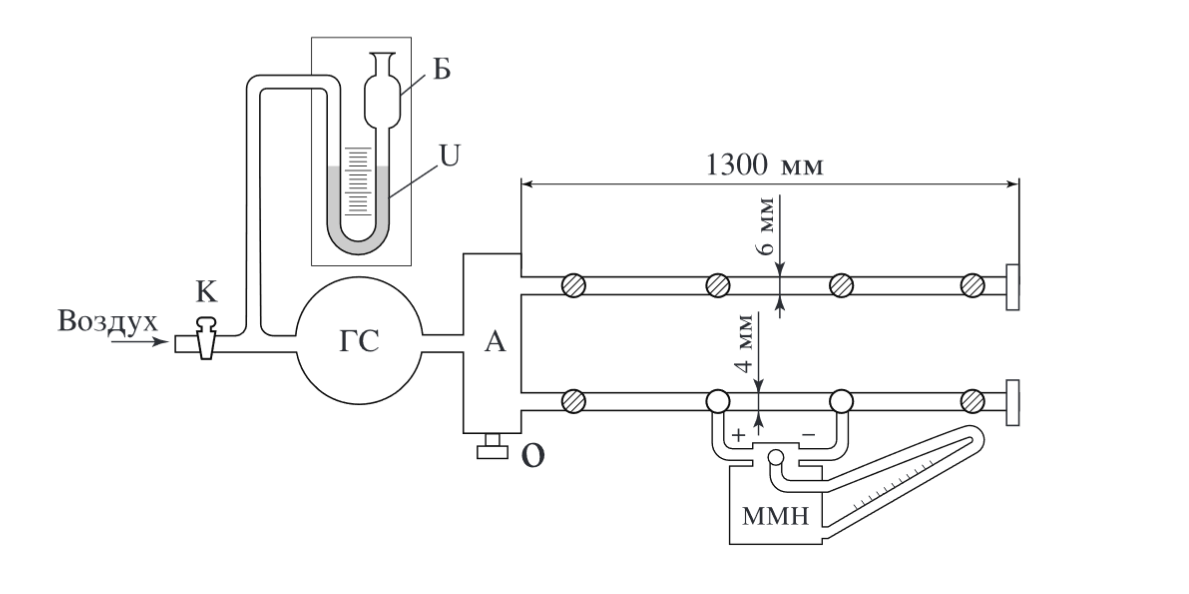
\includegraphics[width = 0.9\linewidth]{instrument}
		Поток воздуха под давлением, несколько превышающим атмосферное(на 5–7 см вод. ст.), через газовый счетчик ГС поступает в резервуар А, к которому припаяны тонкие металлические трубки. Обе трубки на концах снабжены заглушками, не пропускающими воздух . Во время измерений	заглушка открывается только на рабочей трубке; конец другой трубки должен быть плотно закрыт.
		Перед входом в газосчётчик поставлена U-образная трубка, наполовину заполненная водой. Она выполняет две задачи . Первая --- измерение давления газа на входе в газосчётчик. Вторая --- предохранение газосчётчика от выхода из строя. Дело в том, что  газосчётчик	устойчиво  работает, если давление газа на его входе не превышает 600 мм водяногостолба. Высота  U-образной трубки примерно 600 мм, поэтому, когда давление на входе в счётчик превышает 600 мм  водяного столба, жидкость с шумом выплескивается в баллон.					
	\section{Ход работы}
		\subsection{Парметры установки}
			\[
			d_1 = 5.255 \pm 0.005 \, \text{мм} \qquad
			d_2 = 3 \pm 0.1\, \text{мм} \qquad
			d_3 = 3.855 \pm 0.005\, \text{мм} \qquad
			\]
			\[
			P = p_{\text{дел}}\cdot0.2\cdot9.80665
			\]
		\subsection{Измерения}
		Измерим зависимость расхода от перепада давления.
		\begin{center}
			\begin{tabular}{  l | l | l | l }
				$\Delta P$, дел & $\Delta V$, л & $\Delta t$, c & $Q\, \frac{\text{м}^3}{c}\cdot 10^{-5}$ \\ \hline
				15 & 4 & 182 & 2.2 \\ \hline
				30 & 4 & 96 & 4.17  \\ \hline
				45 & 4 & 67 & 5.97 \\ \hline
				60 & 4 & 51 & 7.84 \\ \hline
				75 & 4 & 43 & 9.3 \\ \hline
				90 & 4 & 40 & 10 \\ \hline
				105 & 4 & 38 & 105 \\ \hline
				120 & 4 & 36 & 111  \\ \hline
				150 & 4 & 32 & 125 \\ \hline
				180 & 4 & 30 & 133  \\ \hline
				210 & 4 & 28 & 143 \\ \hline				
			\end{tabular}
		\end{center}
		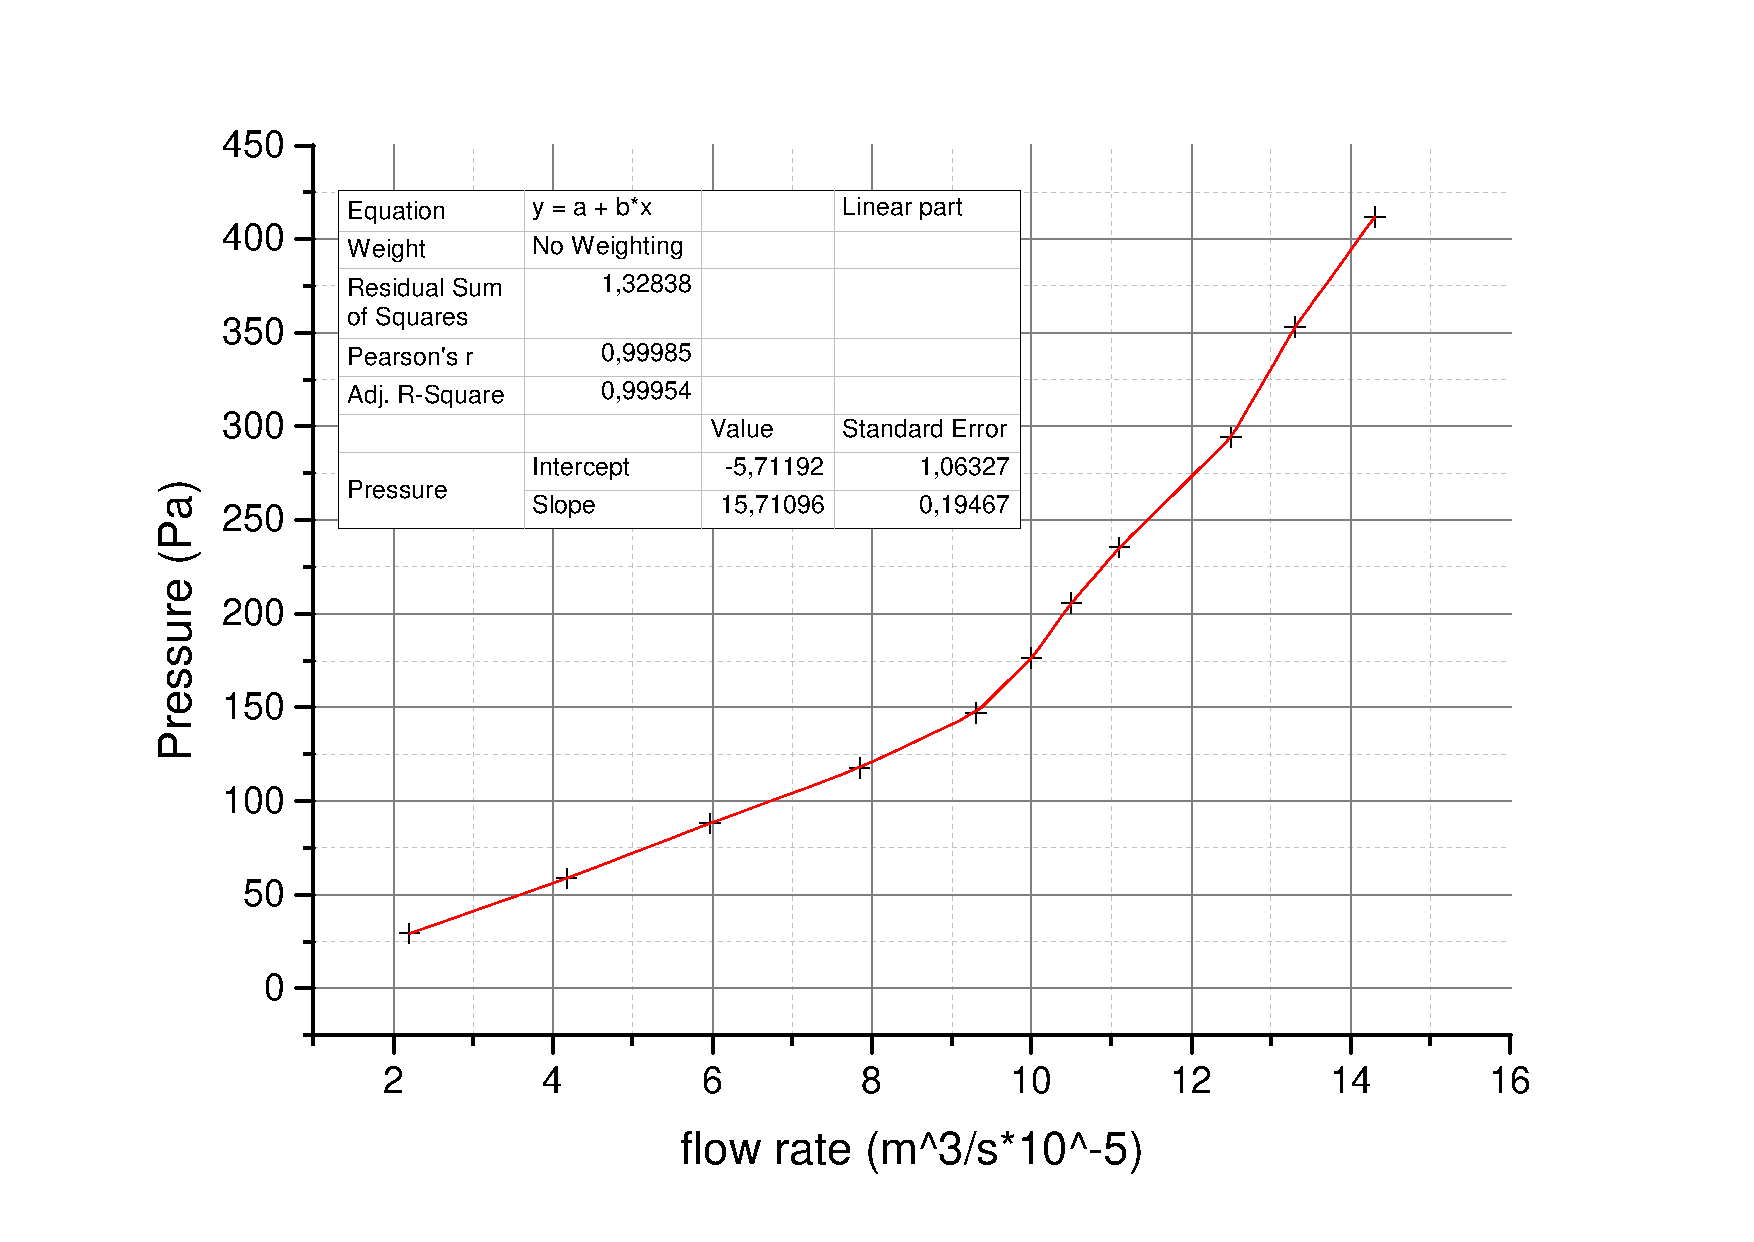
\includegraphics[width = 0.9\linewidth]{graph1}
		
		Вязкость воздуха 
		\[
		\eta = \left(1.86\pm0.02\right)\cdot 10^{-5}\,\text{Па}\cdot\text{c}
		\]
		
		Это значение в пределах погрешности сходится с табличным:
		\[
		\eta_T = 1.85\cdot 10^{-5}\,\text{Па}\cdot\text{c}, \quad T = 25^oC
		\]
		
		Оценим число Рейнольдса, при котором происходит переход к турбулентному течению. Поскольку $V_{\text{ср}}=\frac{Q}{\pi r^2}$.
		\[
		Re= \frac{Q\rho r}{\pi r^2 \eta} = \frac{r^\Delta P}{8 l \eta^2}
		\]
		\[
		Re = \frac{130 \cdot (9\cdot 10^{-5})^3}{8\cdot 0.5 \cdot (1.86\cdot10^{-5})^2} = 670
		\]
		
		
	Измерим распределение давления длине трубы.
	$V = 5\text{л}, t = 179 c$
	\begin{center}
		\begin{tabular}{ l | l | l | l | l | l }
			\multicolumn{2}{c}{$d_1$} & \multicolumn{2}{c}{$d_2$} & \multicolumn{2}{c}{$d_3$} \\ \hline
			P, дел & L, см & P, дел & L, см & P, дел & L, см \\ \hline
			2.5 & 10.5 & 4 & 6 & 10 & 11 \\ \hline
			6.5 & 40.5 & 14 & 26 & 22 & 41 \\ \hline
			12 & 80.5 & 21 & 46 & 39.5 & 81 \\ \hline
			18.5 & 130.5 &  &  & 61.5 & 131  \\ \hline
		\end{tabular}
	\end{center}
	
	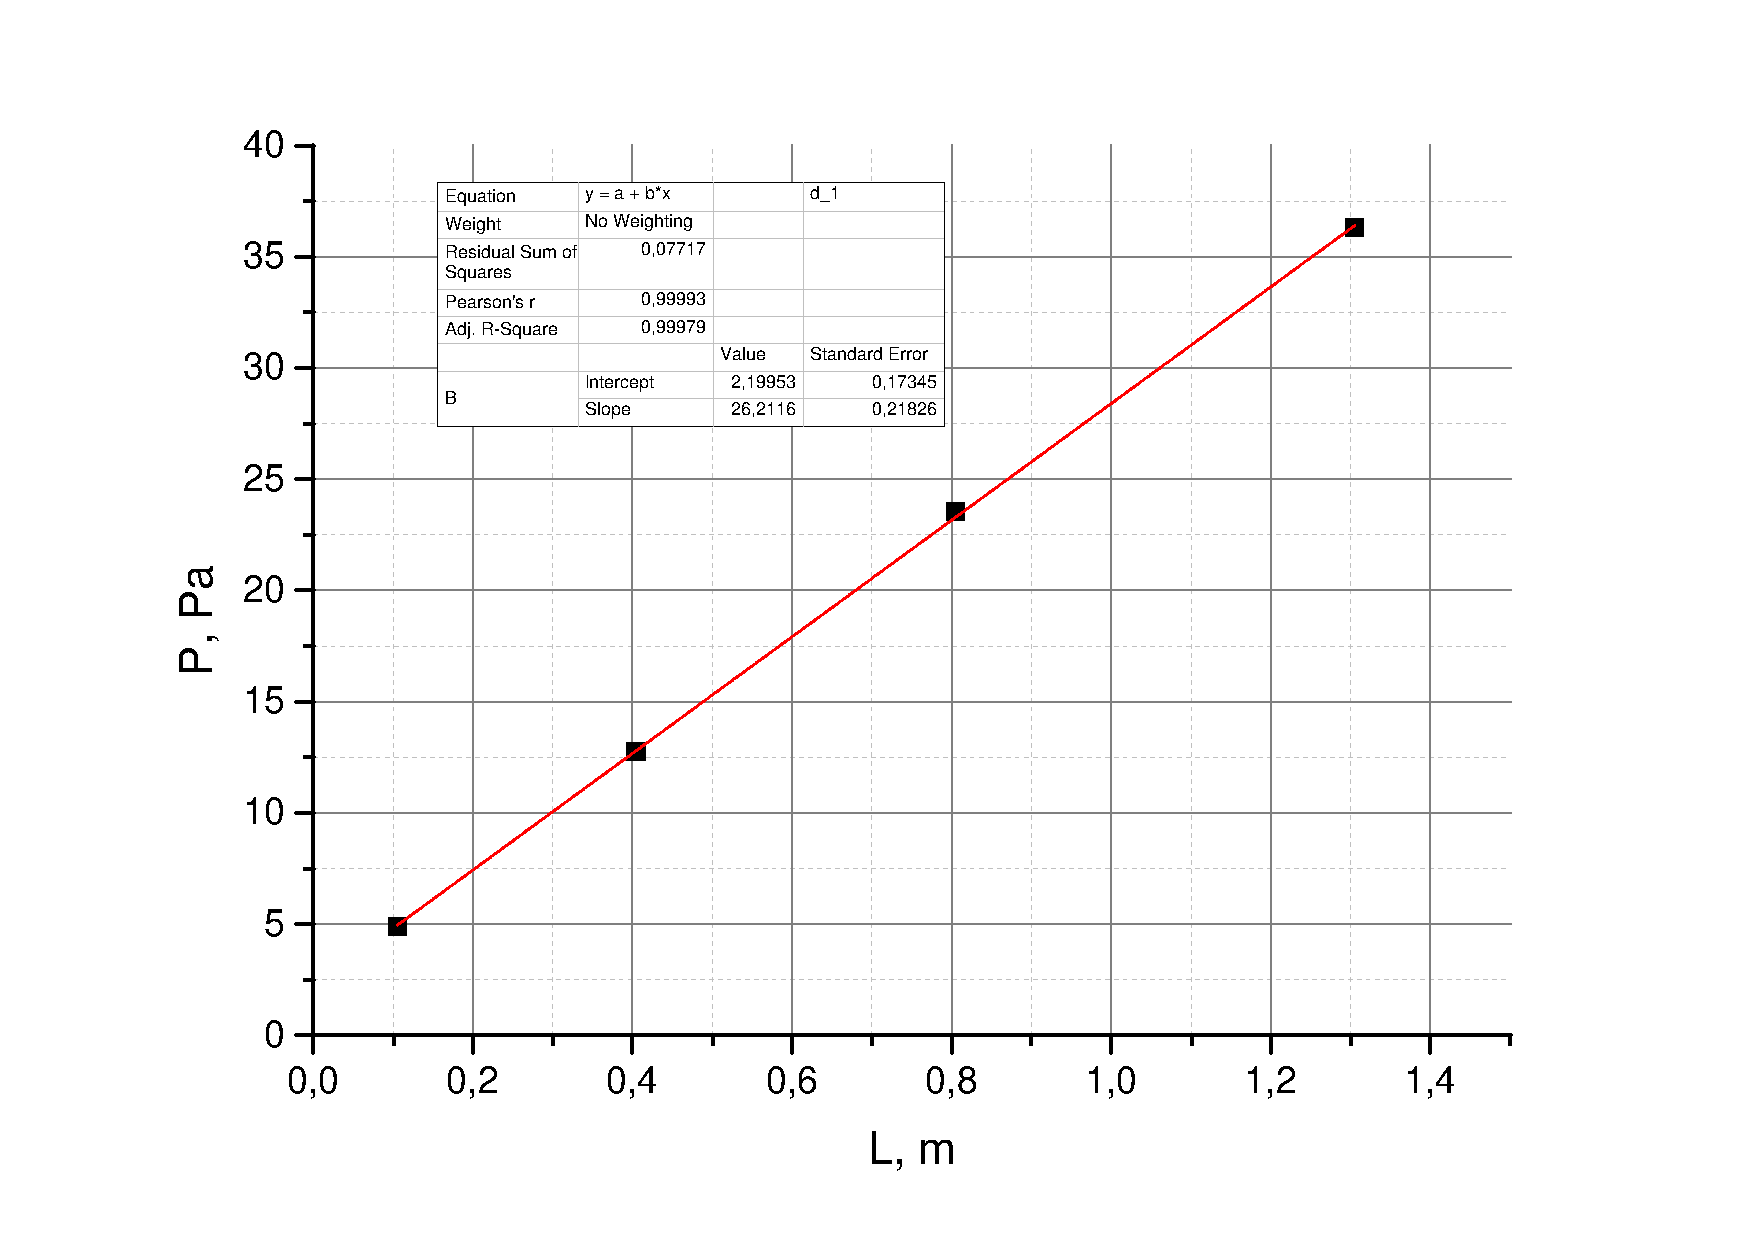
\includegraphics[width = 0.9\linewidth]{Graph2}
	
	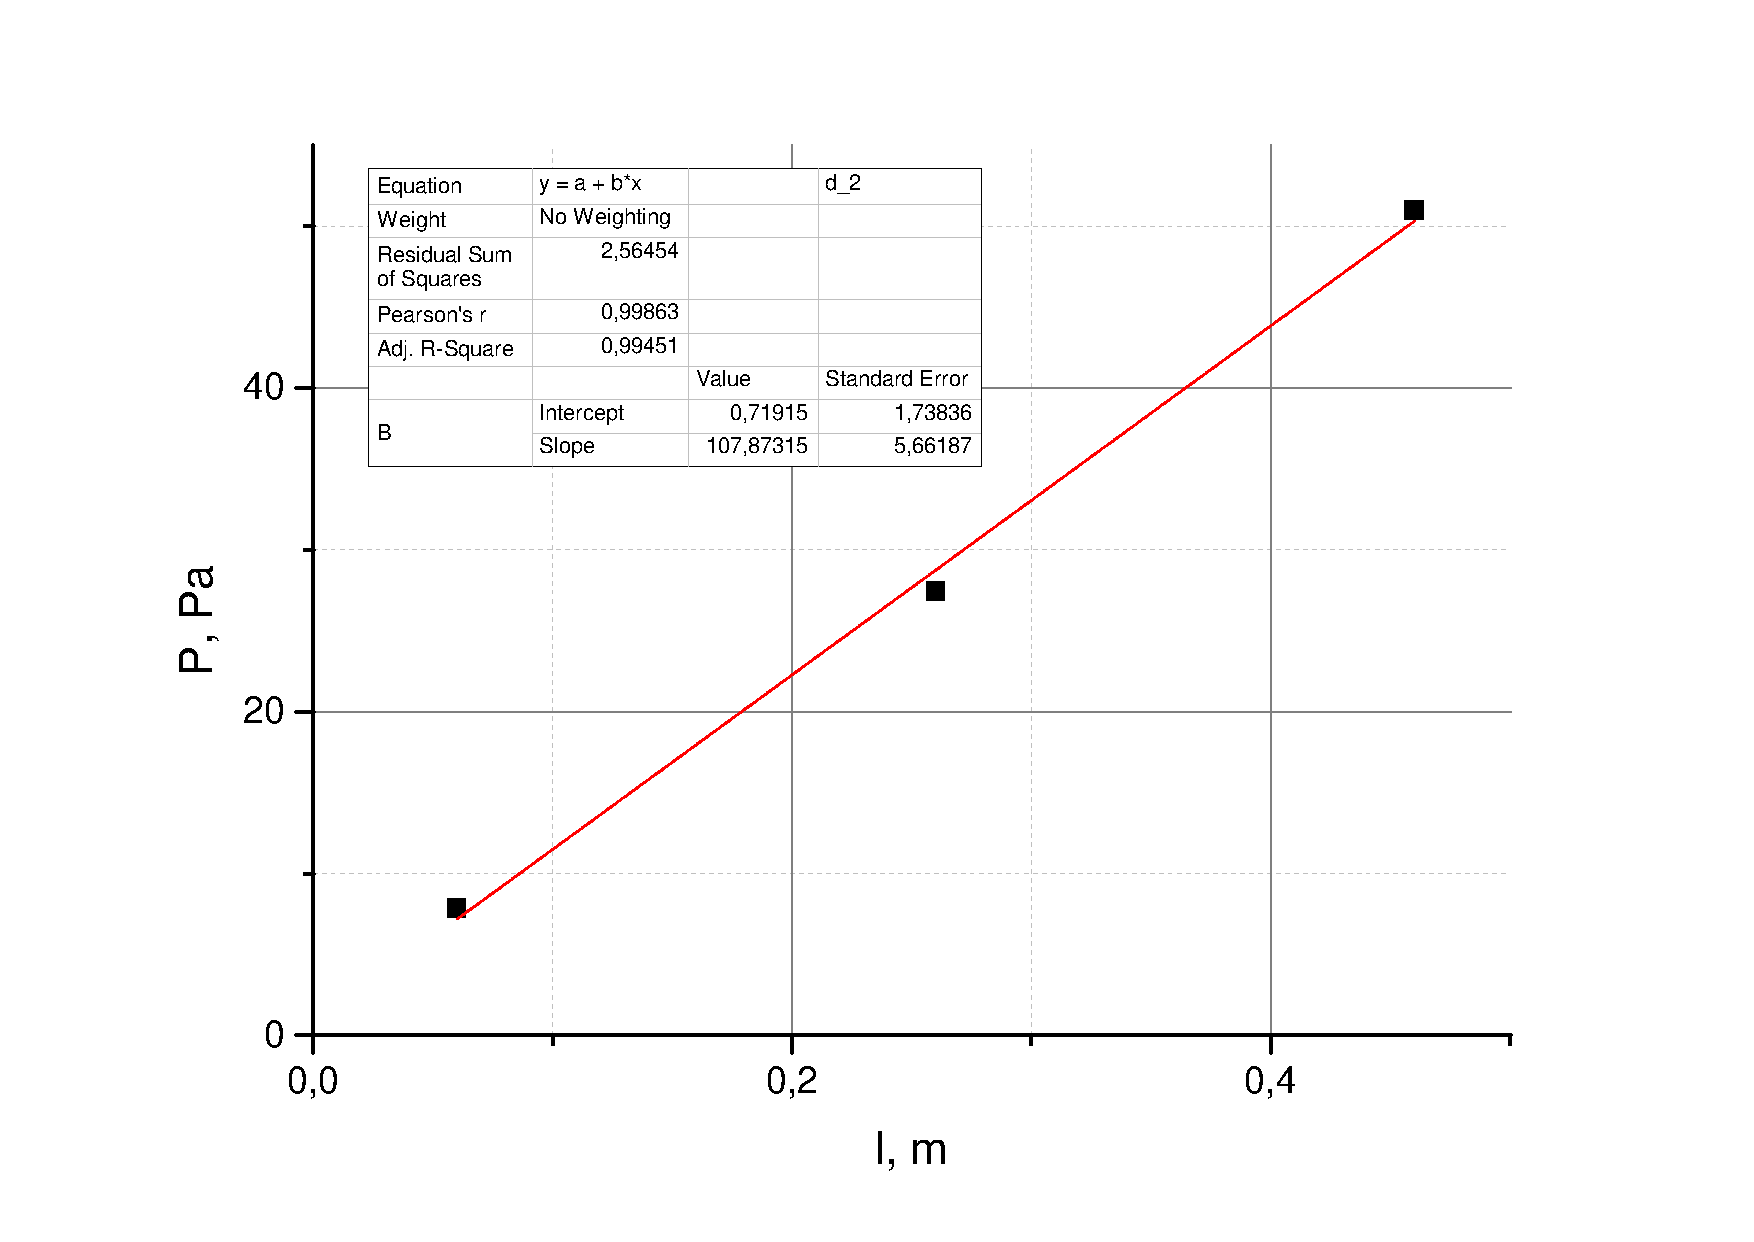
\includegraphics[width = 0.9\linewidth]{Graph3}
	
	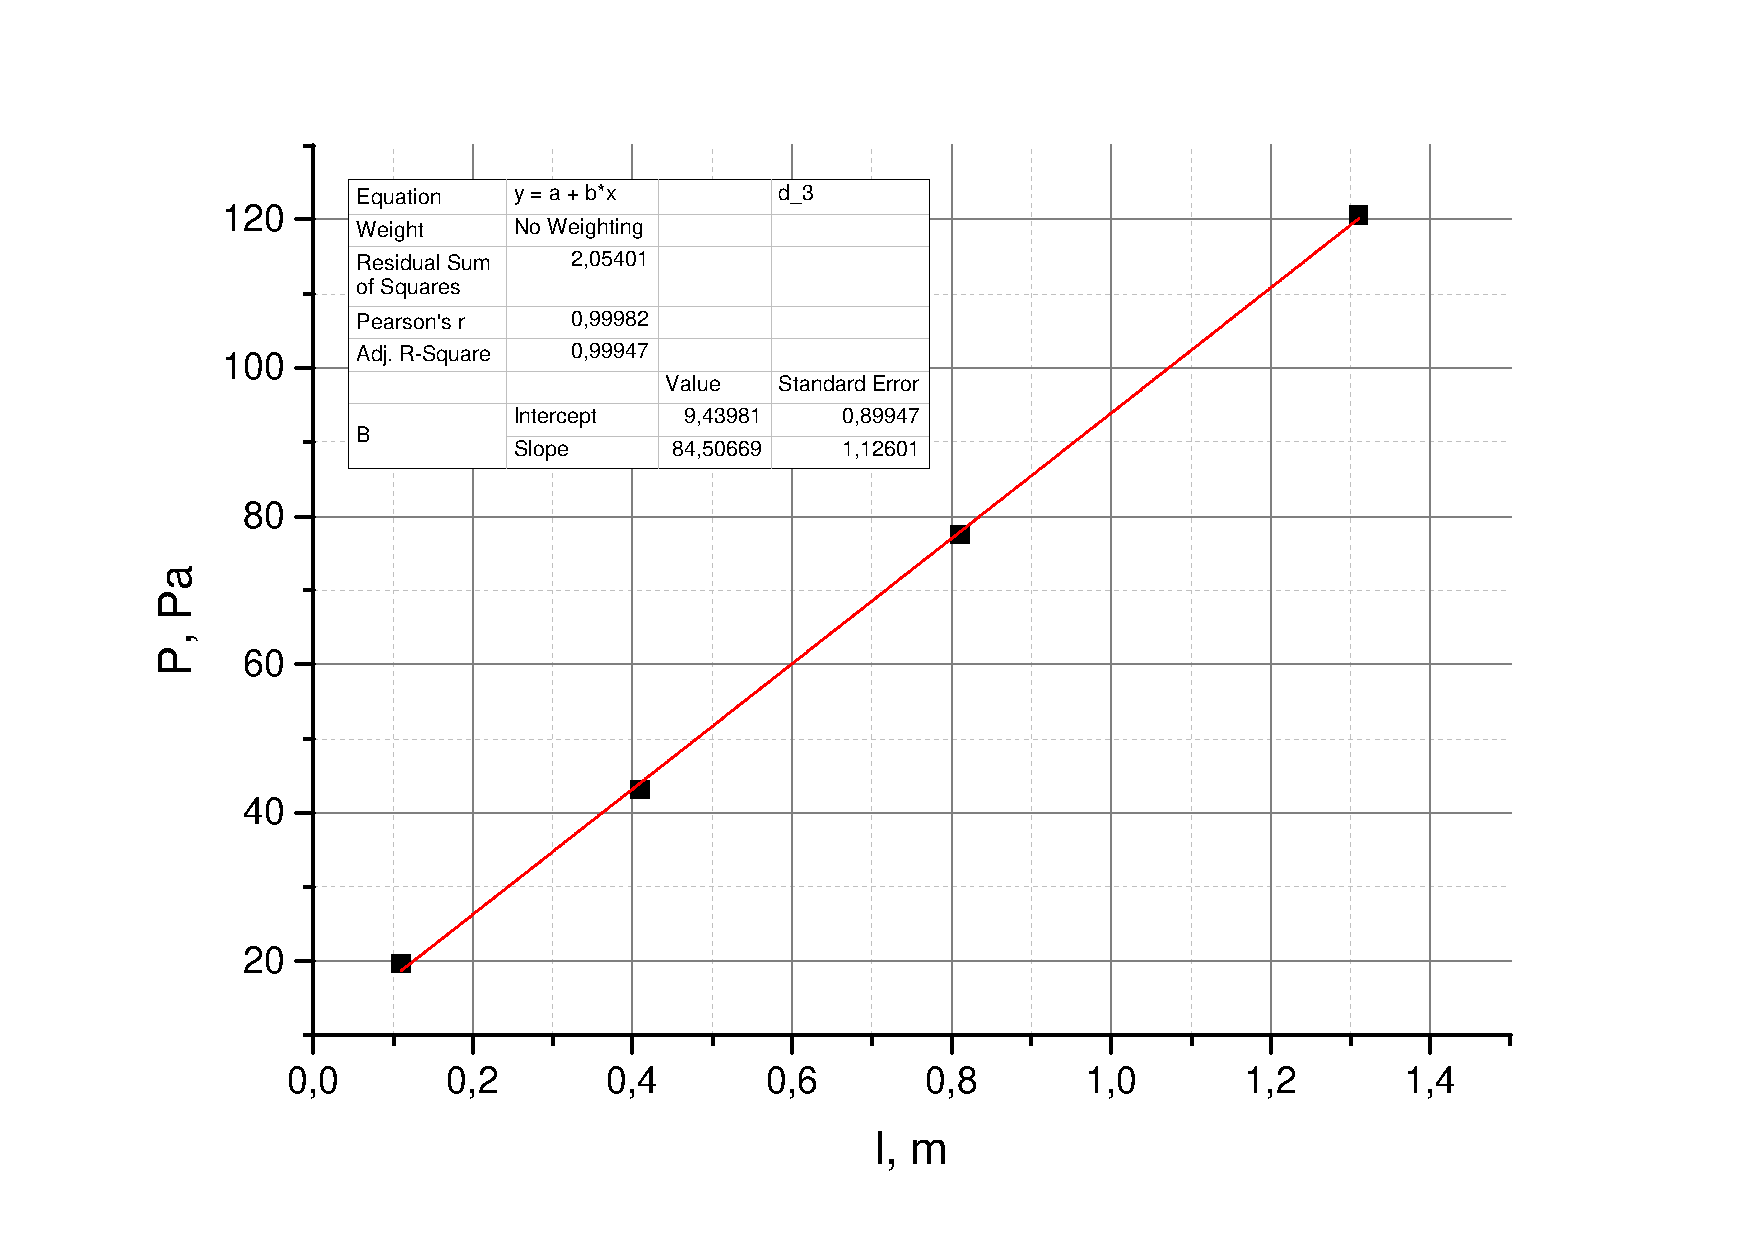
\includegraphics[width = 0.9\linewidth]{Graph4}
	
	
	Построим график в двойном логарифмическом масштабе: по оси ординат отложим $\ln \frac{8l\eta Q}{\pi\Delta P}$, а по оси абсцисс $\ln r$. Угол наклона прямой, очевидно, должен быть равен 4.
	
	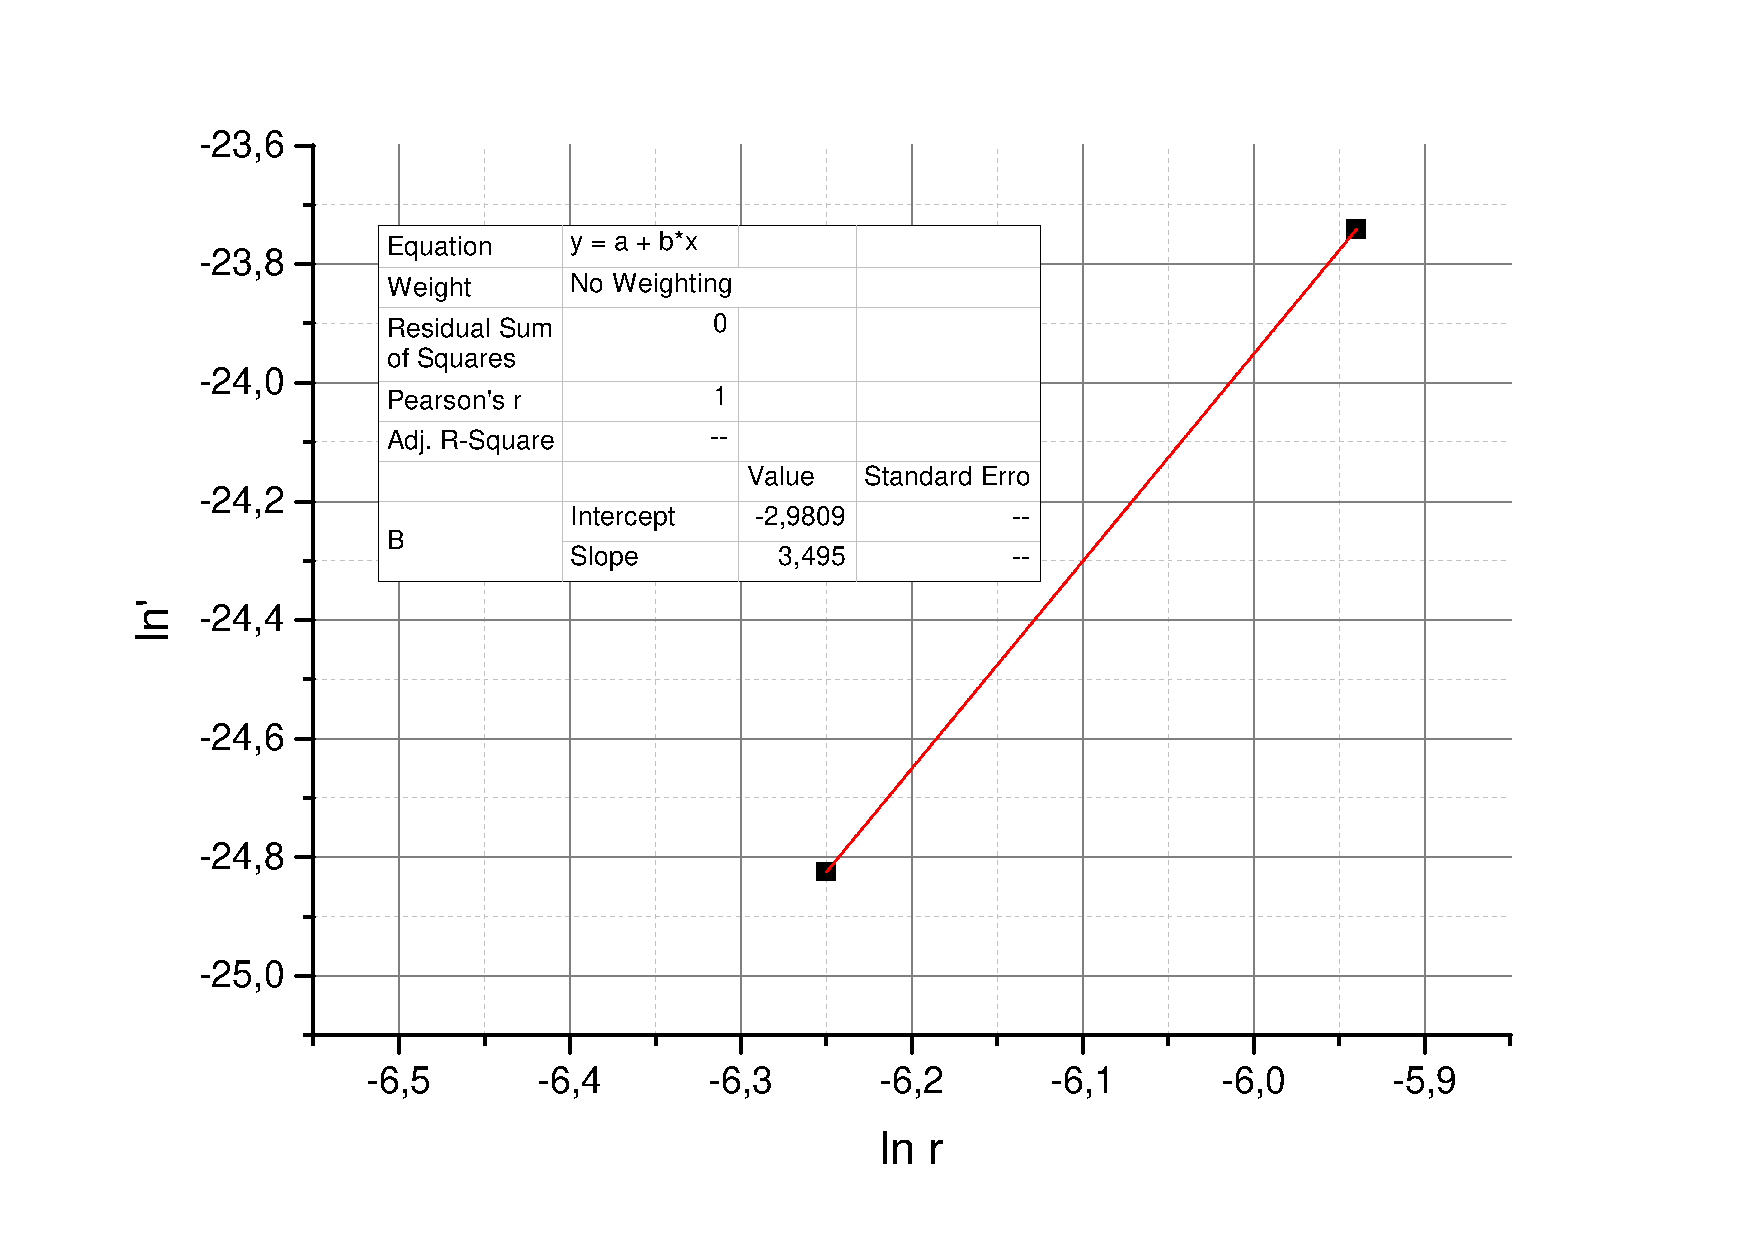
\includegraphics[width = 0.9\linewidth]{Graph5}
	\section{Вывод}
		Измеряя расход газа при течении через тонкие трубки можно установить ламинарность течения, вычислить число Рейнольдса и коэффициент вязкости. Полученный нами коэффициент вязкости сходится с табличным в пределах погрешности, что говорит о высокой точности метода.
\end{document}


